\section{Related Work}




%%%%%%%%%%%%%%%%%%%%%%%%%%%%%%%%%%%%%%%%%%%5
%\begin{figure}[t!]
%  \includegraphics[width=0.5\textwidth]%{figures/qsortps_1GB_nested_precopy_disable_rate_limit.pdf}
  %\caption{Performance of QuickSort }
  %\label{quicksort-performance-1GB-nested-vhost-vhost.png}
%\end{figure}

%\begin{figure}[t!]
%  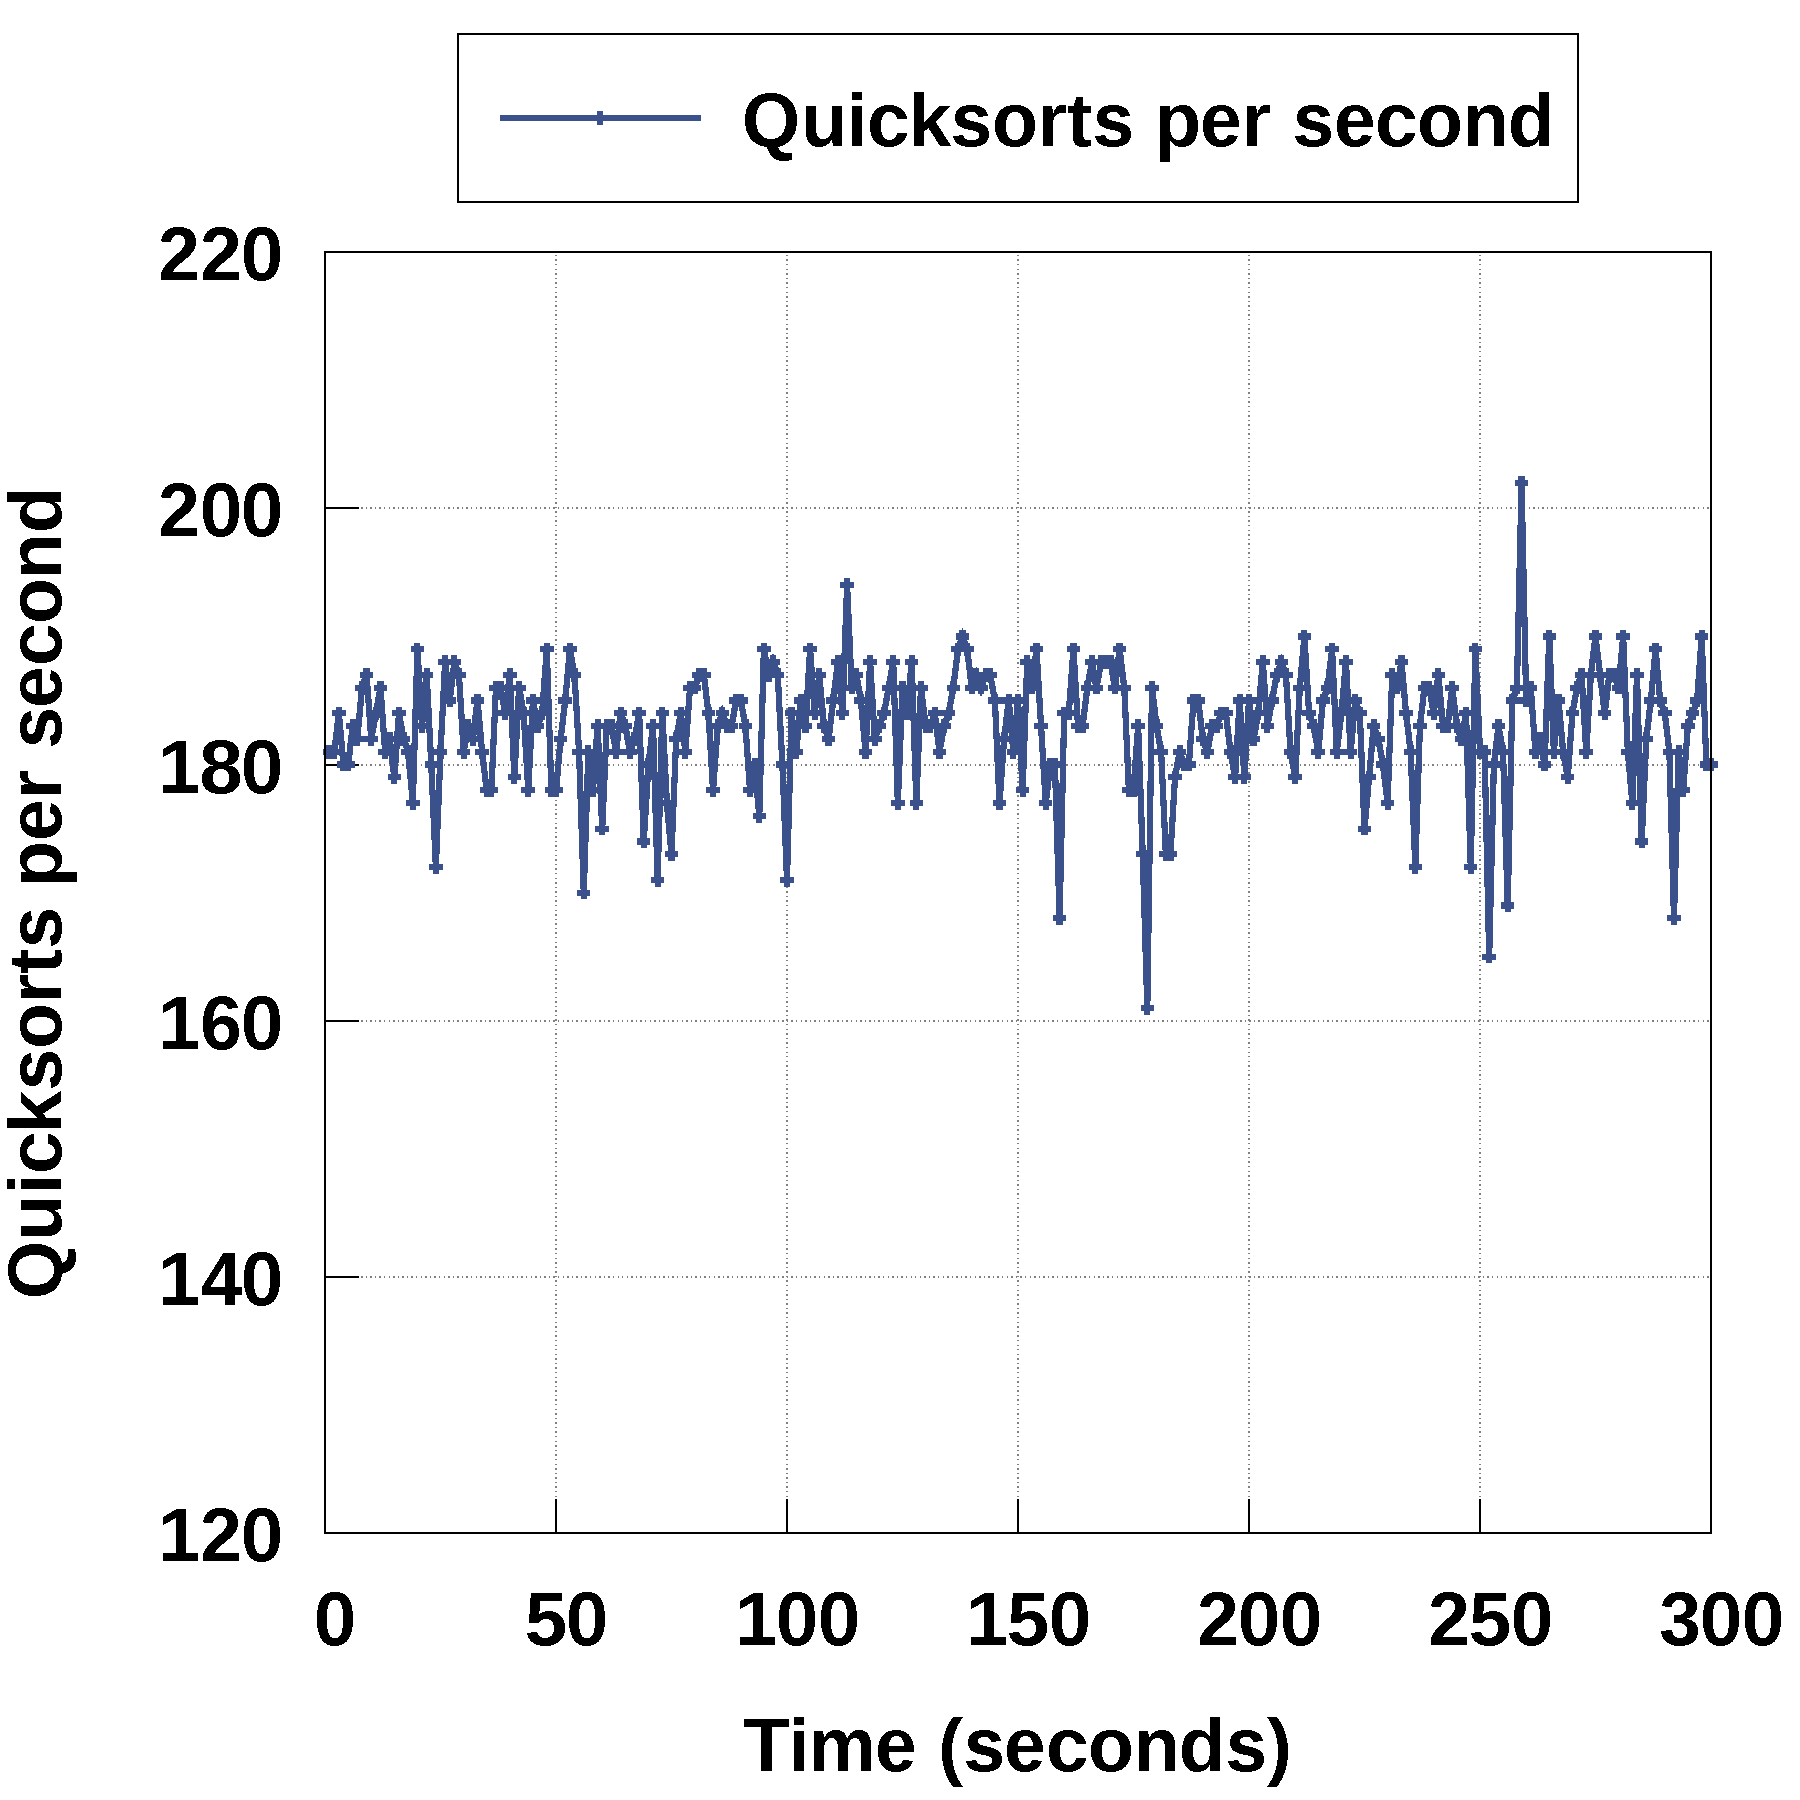
\includegraphics[width=0.35\textwidth]{figures/qsortps_1GB_nested_precopy_hyperfresh.pdf}
  %\caption{Performance of QuickSort during migration of a nested guest}
%  \label{quicksort-performance-1GB-nested-vhost-vhost.png}
%\end{figure}

%\begin{table*}\centering

%\begin{tabular}
%{|p{4cm}|p{1cm}|p{1cm}|p{1.5cm}|p{1.5cm}|p{1.5cm}|p{1.5cm}|p{1.5cm}|} \hline
% & & & & & \multicolumn{3}{c|}{\% Overhead vs. Host} \\ \cline{6-8} 
%Benchmark & Host & Non-nested Guest & Nested Guest & Our Solution & Non-nested Guest & Nested %Guest & Our Solution \\ \hline
%iPerf Bandwidth (Gbps) - Server & 37.6 & 29.9 & 25.2 & 29.7 & 20.5 & 32.97 & 21 \\ 
%iPerf Bandwidth (Gbps) - Client & 37.6 & 36.3 & 26.6 & 36.1 & 3.45 & 29.25 & 3.98 \\ \hline
%Kernbench Runtime (seconds) & 37.47 & 38.51 & 40.52 & 40.32 & 2.8 & 8.1 & 7.6 \\ \hline
%Quicksort Runtime (useconds) & 66.29 & 66.51 & 67.77 & 67.57 & 0.3 & 2.23 & 1.9 \\ \hline
%
%\end{tabular}
%\vspace{6pt}
%
%\caption{Comparison of performance overhead due to virtualization}
%\label{Comparison of performance overhead due to virtualization}
%\end{table*}

%\begin{table*}\centering
%\begin{tabular}{|p{4.5cm}|p{0.8cm}|p{0.8cm}|p{0.8cm}|p{0.8cm}|p{0.8cm}|p{0.8cm}|p{0.8cm}|p{0.8cm}|p{0.8cm}|p{0.8cm}|} \hline
%    \multirow{1}{*}{} & &
%      \multicolumn{9}{c|}{CPU Utilization} \\ \cline{3-11}
%    \multirow{1}{*}{} & Guest &
%      \multicolumn{3}{c|}{Hyperplexor} & 
%      \multicolumn{3}{c|}{Hypervisor} & 
%      \multicolumn{3}{c|}{Guest} \\ \cline{3-11}
 
%\textbf{} & & User & System & Guest & User & System & Guest & User & System & Guest \\ \hline
%\multirow{ 2}{5cm}{Non-nested guest (paravirt)} & Server & 114.63 & 247.09 & 114.63 & - & - & - & 1.8 & 91.7 & 0 \\ 
%& Client & 114.4 & 122.7 & 114.3 & - & - & - & 1.18 & 84.64 & 0 \\ \hline

%\multirow{ 2}{5cm}{Nested Guest (passthrough-paravirt)} & Server & 253.1 & 308.3 & 252.9 & 91.18 & 150.72 & 90.9 & 1.9 & 107.18 & 0\\ 
%& Client & 126.3 & 205.7 & 126.5 & 82.72 & 107.54 & 82.63 & 0.63 & 121.17 & 0 \\ \hline

%\multirow{ 2}{5cm}{Nested Guest (passthrough-paravirt) + Optimizations} & Server & 265.7 & 85.5 & 265.7 & 116.2 & 143.1 & 116.45 & 2.45 & 118.44 & 0 \\ 
%& Client & 195.6 & 93.5 & 195.6 & 95.54 & 93.18 & 95.27 & 1.17 & 135.8 & 0 \\ \hline

%\end{tabular}
%\vspace{6pt}
%\caption{CPU Utilization}
%\label{CPU Utilization}
%\end{table*}


%\begin{table}
%\begin{tabular}{|p{3.2cm}|p{2.0cm}|p{2.0cm}|} \hline
% & \multicolumn{2}{|c|}{\textbf{Number of VM Exits}} \\ \cline{2-3} 
%\textbf{VM Exit Reasons}& \textbf{Before optimizations} & \textbf{After optimizations}\\ %\hline
%\textbf{HLT} & &\\ \hline
%\textbf{MSR\_WRITE} & &\\ \hline
%\textbf{EXTERNAL\_INTERRUPT} & &\\ \hline
%\textbf{PREEMPTION\_TIMER} & &\\ \hline
%\textbf{IO\_INSTRUCTION} & &\\ \hline
%\textbf{EXCEPTION\_NMI} & &\\ \hline
%\textbf{PAUSE\_INSTRUCTION} & &\\ \hline
%\textbf{EPT\_VIOLATION} & &\\ \hline
%\textbf{MSR\_READ} & &\\ \hline
%\textbf{CPUID} & &\\ \hline
%\textbf{TOTAL} &  &\\ \hline
%\end{tabular}
%\vspace{6pt}
%\caption{VM Exit Reasons}
%\label{VM Exit Reasons}
%\end{table}
 
%\begin{document}

Software aging \cite{parnas1994software} is the phenomenon where
software errors, such as  memory leaks, accumulate over time,
leading to performance degradation or complete system failure.
Software Rejuvenation \cite{huang1995software} is a proactive technique where 
the system is periodically restarted to a clean internal state to
counter software aging. In cloud environments, software aging 
of hypervisors and OS is of utmost concern, where the impact of 
their failures could be widespread.

In cold rejuvenation of hypervisors, all VMs must be restarted
whereas in warm rejuvenation the VMs' memory state is preserved 
in persistent memory and restored after hypervisor rejuvenation, 
avoiding costly read/writes to persistent storage. 
Roothammer \cite{kourai2007fast} proposed warm reboot to rejuvenate 
a Xen hypervisor 
%which avoids cache-misses by preserving the 
VM images in main memory reducing the VM reboot time. 

A simpler approach is to live migrate the VMs to a different host. 
Live migration~\cite{clark2005live, postcopy} reduces the downtime 
by letting the virtual machines run when the memory is copied in 
multiple rounds to another host. However, live migration also incurs 
network overhead as large quantities of memory is transferred. 
In this paper, we eliminate the memory copies for intra-host VM/container 
migration by page relocation on the same host. 
%We also eliminate multiple copies of VM images as the hypervisor replacement happens on the same machine. 
ReHype \cite{le2011rehype} performs a microreboot~\cite{candea2004microreboot} of 
the hypervisor by preserving the state of the VMs. The state of 
the rebooted hypervisor is then re-integrated with the state of the preserved VMs. 
Since this reintegration depends heavily on the hypervisor's state,
the success rate is low.   
Kourai et. al proposed VMBeam \cite{kourai2015zero}
where a clean virtualized system is started and all the 
virtual machines are migrated from old virtualized system to new one 
with zero-memory copy. Unlike our approach, VMBeam takes 16.5 seconds 
to migrate a 4 GB VM with zero memory copy, potentially due to 
non-live or inefficient transfer of memory maps. 
HyperFresh~\cite{hyperfresh_apsys} also uses memory co-mapping  to
replace a stale hypervisor with a fresh one. However, the refresh times 
are close to 100 ms for relocating a single VM, and multiple VMs relocation
is not addressed. Finally, unlike the above approaches, our \arch
addresses reduction of nesting overheads during normal execution
and live OS replacement for processes and containers.

%Remus \cite{cully2008remus} is a reactive technique that achieves high availability by periodically checkpointing the VM image and incrementally storing the changes in the memory of backup host. On failure of current host, the VM can be immediately started on the backup host using the checkpointed memory. The VM images along with network and disk state are checkpointed as frequently as 25ms. To transfer the incremental changes in the VM’s memory, it requires higher network bandwidth. The traffic generated over the network results in performance degradation of the applications running in the virtual machines. VMWareFT \cite{scales2010design} uses deterministic replay to keep both primary and backup VMs in sync. Again it requires high quality network connections. In our technique, we transfer only the processor and the I/O state during hypervisor replacement through the network. As shown in the evaluation section, it does not affect the performance of the applications running in the VM. Upon encountering an error in the hypervisor, 

Applying updates to an OS kernel comes with high cost of downtime due to system reboot. 
Kernel patching is a complex process of replacing original outdated functions or 
data structures with new ones. Ksplice \cite{arnold2009ksplice}, Kpatch \cite{kpatch1, kpatch2}, 
Kgraft \cite{kgraft} follow the mechanism of replacing old vulnerable functions with 
new functions using ftrace mechanism. Kpatch and Ksplice stop the machine to check 
if any of the threads is executing in the function to be patched. If any of the processes 
is executing or is sleeping in the function to be patched, the kernel patching is retried later 
or called off after several attempts. Kgraft keeps a copy of both old and new functions. 
If the kernel code is active during patching, it runs till completion before switching to 
the new functions while the other processes use the updated functions. 
Live patching \cite{livepatch} is a combination of Kpatch and Kgraft kernel patching 
methods. Kernel patching technique can be useful for applying simple 
fixes to delay system failure until the next maintenance period, 
but it still requires an OS reboot at some stage. 
Major changes to the kernel also require immediate reboot to take effect. 
Further these techniques cannot patch asm, vdso, or functions that cannot be traced.
In contrast, \arch bypasses these problems by remapping the memory of
containers/processes to a fresh co-located instance of the kernel.

Process/container live migration techniques have also been extensively studied 
\cite{spin, exokernel, synthetix, baraks, zayas, douglis, theimer, lsf, condor, criu},
but all require the transfer of the memory contents via network. 
\arch combines memory remapping with intra-host process migration used by CRIU~\cite{criu}
to eliminate memory copying, making it suitable for fast and live OS replacement.

%In general, process migration can be implemented either in the kernel level or in the user level. Kernel level process migration techniques \cite{spin, exokernel, synthetix, baraks, zayas, douglis, theimer} are implemented either with kernel-level inherent support or by modifying the existing operating systems adding complexity. In contrast, user-level implementation \cite{lsf, condor, criu, Amoeba, Chorus, Mach} requires either to modify applications reducing the transparency or to heavily intrude processes for collecting state facing performance degradation. The performance overhead of user-level implementations can be significantly mitigated with key kernel-level support such as exposing as much state information of processes as possible to the user space and/or providing efficient ways to mark dirty pages and transfer them \cite{condor, lsf, criu}. As a container consists of a hierarchy of processes as well as mechanisms that enable isolation and security between containers, state-of-the-art container migration approaches  \cite{docker, openvz, coreos_rocket} build upon process migration. For example, the migration of Docker container \cite{docker} builds on CRIU's \cite{criu} process checkpointing and restoring mechanisms. 

%\para{Live Migration.} A lot of live migration techniques have been proposed.  One approach is post-copy technique \cite{Hines:2009:PLM:1618525.1618528, zayas}, where pages are migrated only when they are referred on the destination machine. Although such an on-demand page migration reduces the initial cost of the migration, it increases the total migration time. Pre-copy \cite{theimer} keeps processes/containers running on the source machine while its memory keeps getting transferred to the destination in an iterative manner; once the dirtied pages are small enough, the whole process is paused and the remaining pages are transferred. If the page dirtying rate is very high, the migration will take way longer to complete. There has also been work that combines some features of these techniques \cite{lazo, loubutin, sinha, dediu, dijk,schill,petri,schrimpf} . For example, instead of copying entire memory state in the most basic technique, only the minimal dirty pages are transferred \cite{roush}. The remaining pages are transferred while the process is running on remote machine. This reduces the transfer cost, but requires the support of the remote paging mechanism. MOSIX \cite{mosix} and Sprite \cite{sprite} implements migration by leaving residual dependencies on the source machine. Although, it makes the migration simple but it requires the source machine to be available all the time till the process completes its execution. 


%\begin{figure}[t!]
%  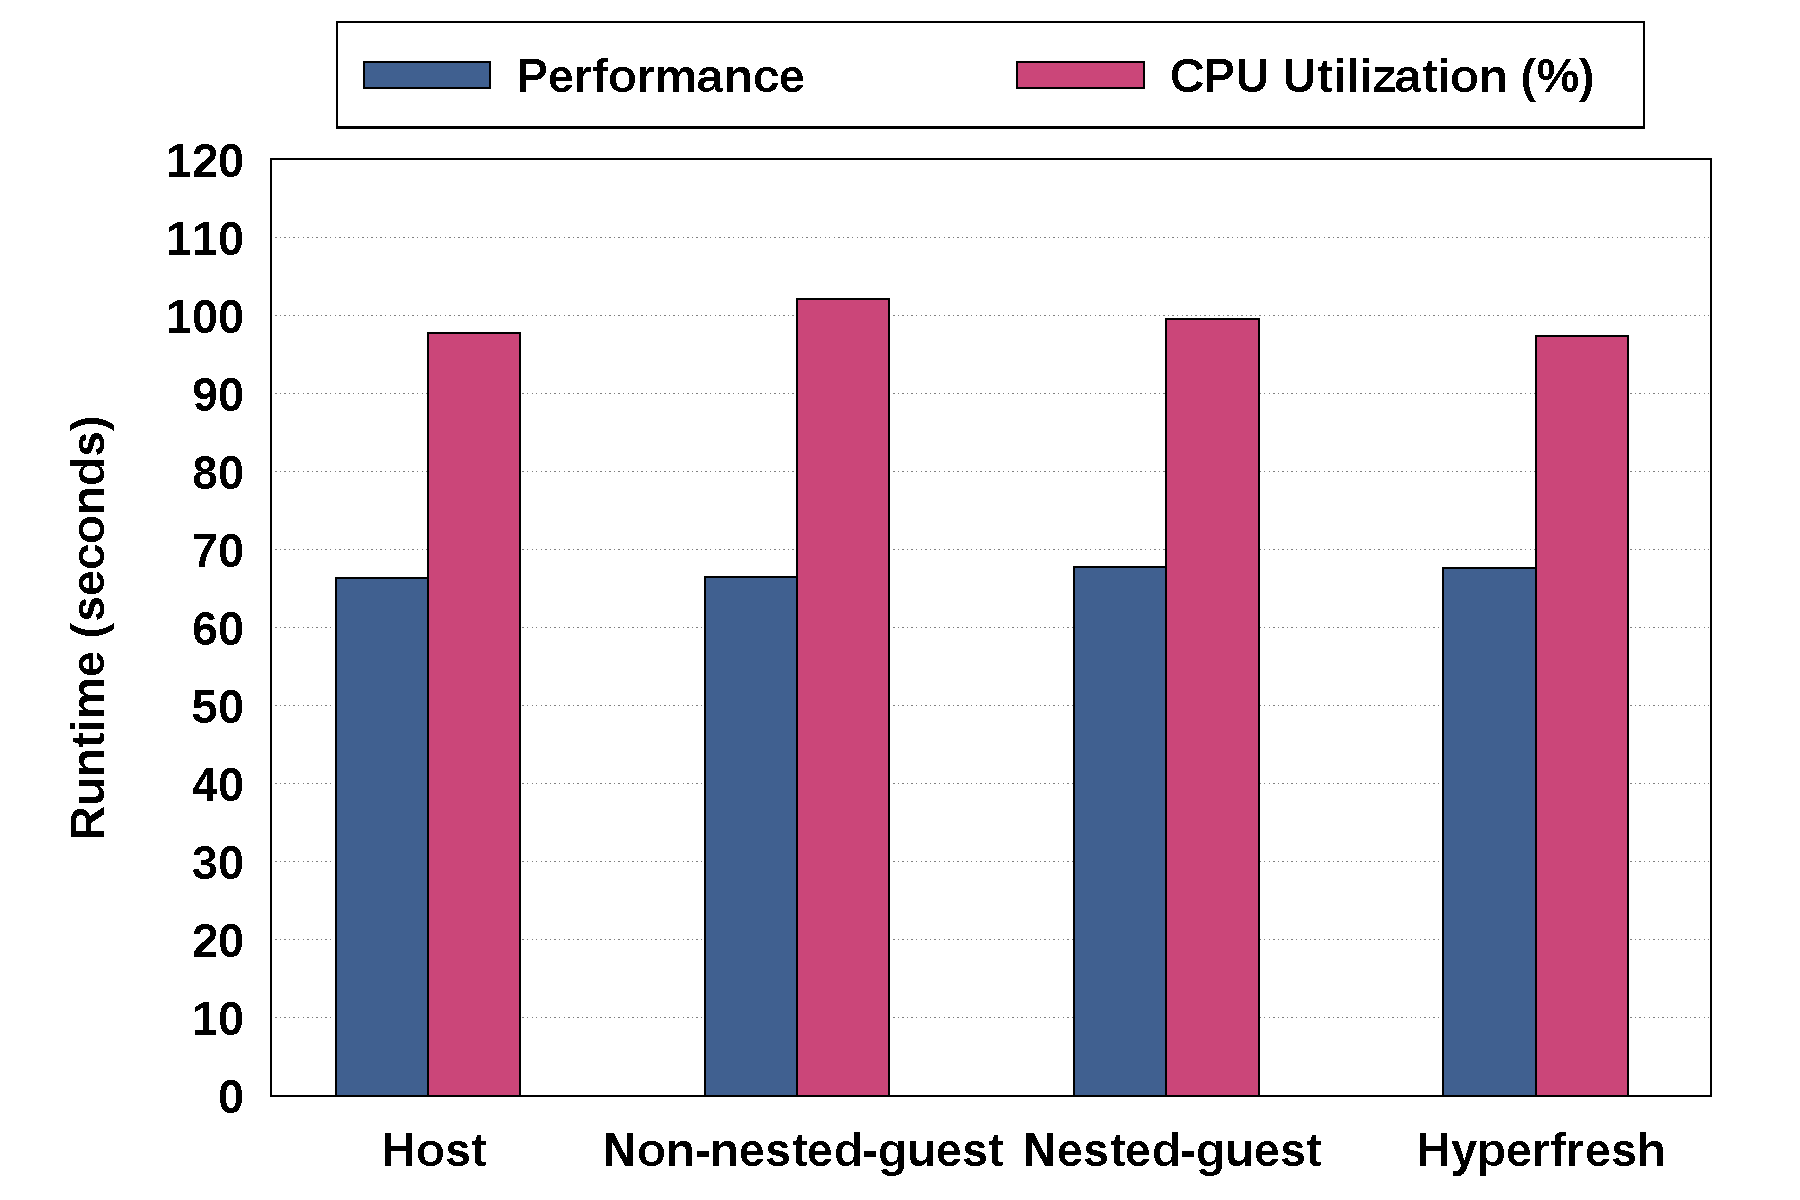
\includegraphics[width=0.5\textwidth]{figures/quicksort.pdf}
%  \caption{Quicksort performance}
%\end{figure}

%\begin{figure}[t!]
%  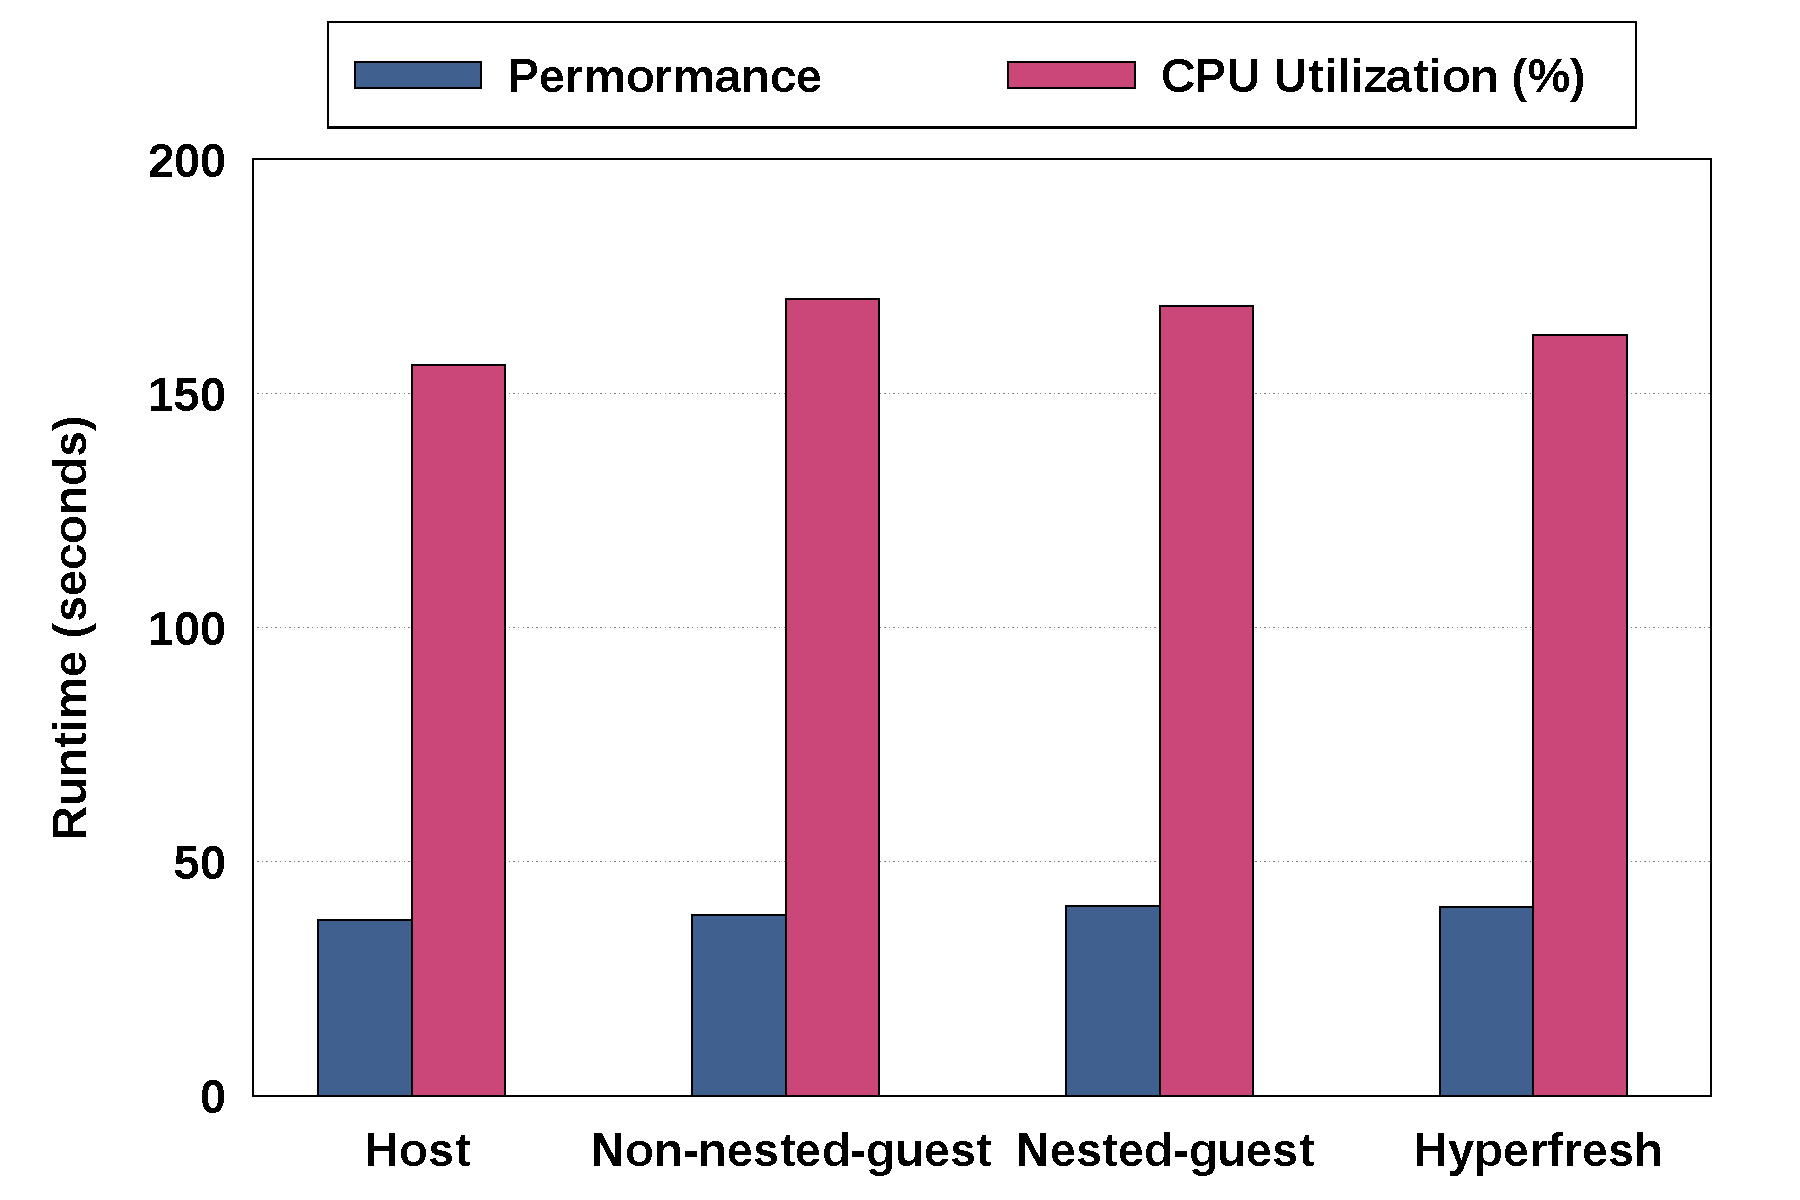
\includegraphics[width=0.5\textwidth]{figures/kernbench.pdf}
%  \caption{Kernbench performance}
%\end{figure}

%\begin{figure}[t!]
%  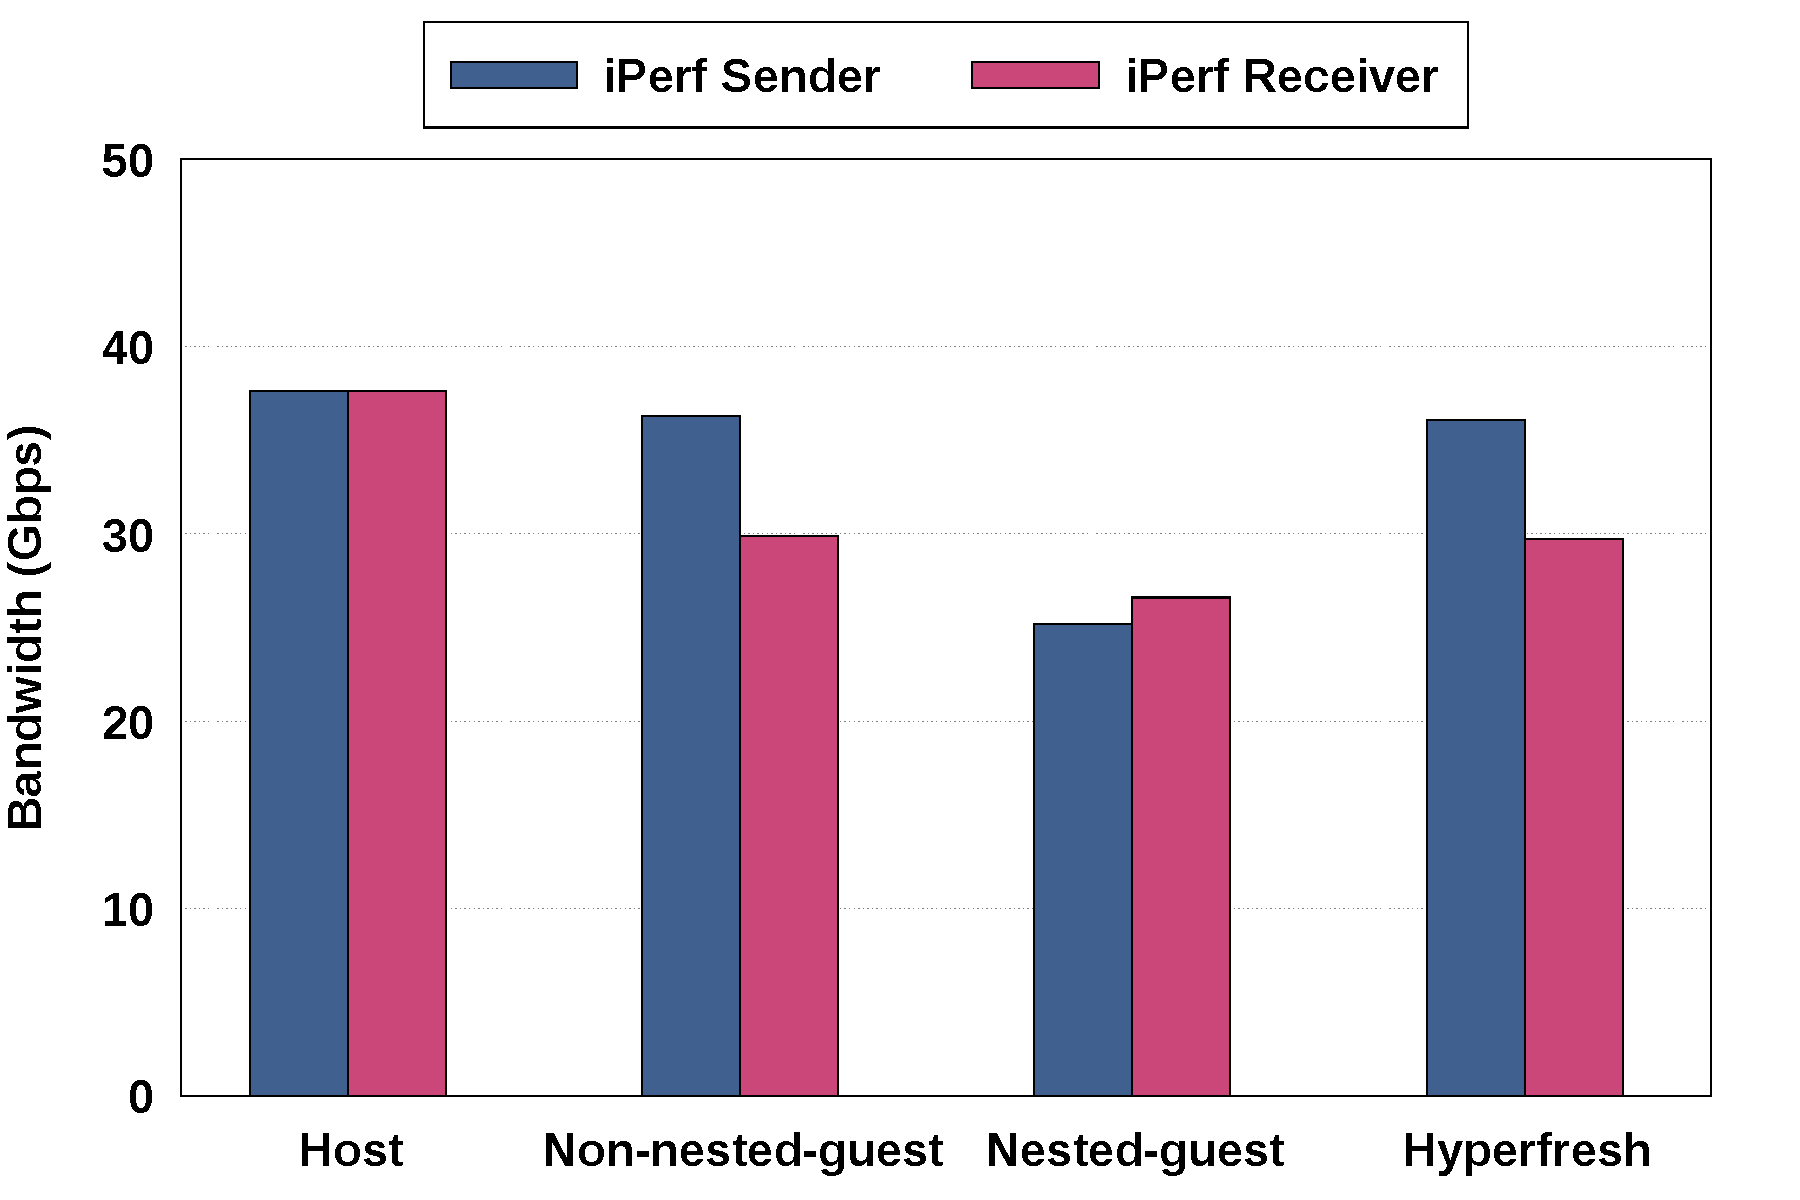
\includegraphics[width=0.5\textwidth]{figures/iperf.pdf}
%  \caption{iPerf performance}
%\end{figure}


%SENDER: 36.1 Gbps RECEIVER: 29.7 Gbps
